\documentclass[UTF8]{ctexart}

\usepackage{graphicx}
\usepackage{amsmath}
\usepackage{amssymb}

\usepackage{listings}
\usepackage{xcolor}


\lstset{
    basicstyle          =   \sffamily,          % 基本代码风格
    keywordstyle        =   \bfseries,          % 关键字风格
    commentstyle        =   \rmfamily\itshape,  % 注释风格,斜体
    stringstyle         =   \ttfamily,  % 字符串风格
    flexiblecolumns,                % 未知
    numbers             =   left,   % 行号的位置在左边
    showspaces          =   false,  % 是否显示空格
    numberstyle         =   \zihao{-5}\ttfamily,    % 行号的样式
    showstringspaces    =   false,
    captionpos          =   t,      % 这段代码的名字所呈现的位置,t for top.
    frame               =   lrtb,   % 显示边框
    language            =   C++,
    keywordstyle        =   \color{blue},
    commentstyle        =   \color{green},
    stringstyle         =   \color{brown},
}

\title{人工智能实验报告01\normalsize使用遗传算法解方程}
\author{116132019089 沈仕越}
\date{\today}

\begin{document}
\maketitle

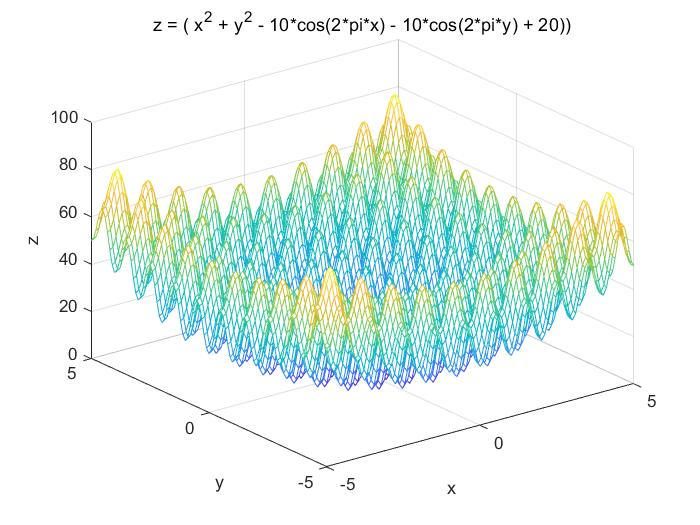
\includegraphics[width = 0.8\textwidth]{func.jpg}
\newpage

\tableofcontents
\newpage

\section{实验目的}
实现使用遗传算法解下面方程:

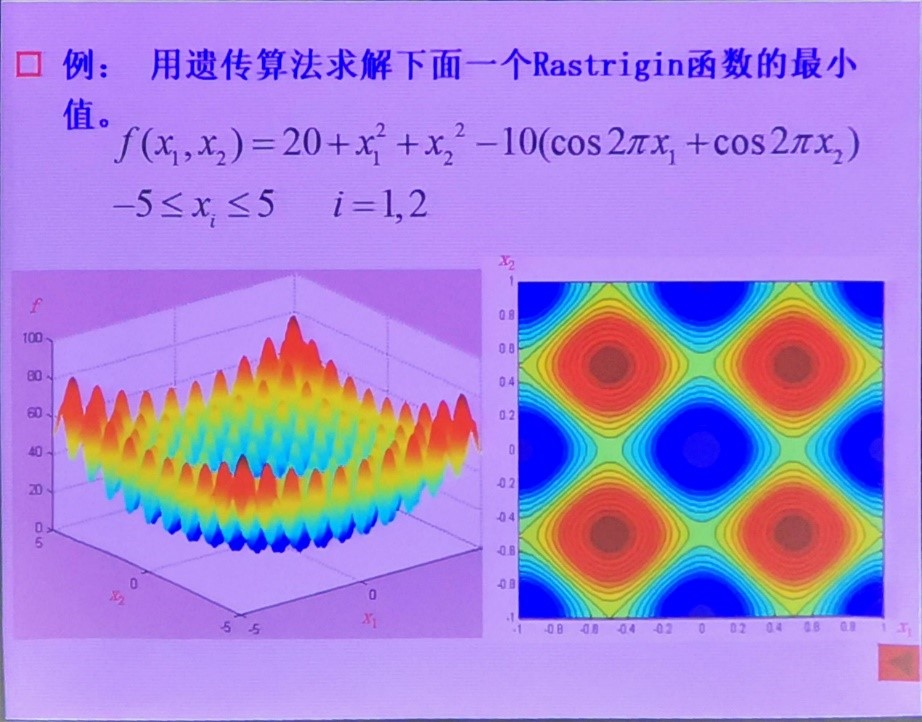
\includegraphics[width = 0.8\textwidth]{problem.jpg}

\section{实验平台}

\begin{enumerate}
    \item 操作系统:Microsoft Windows 10
    \item 编辑器:Microsoft vscode
    \item 编程语言:C++
    \item 编译器:g++
    \item 编译标准:C++11
\end{enumerate}


\section{实验过程}

遗传算法是一种搜索算法,基本思想是使用计算机模拟生物进化的过程,
并通过这种模拟方式在搜索域中寻找出最优解。

遗传算法将问题的解抽象成为基因(或称染色体),并让这些基因按照一定规则进行交叉、
突变、自然选择等,使种群向更优解进化。

进化的过程即是迭代的过程,每一次迭代,算法都会根据某个\textbf{适应性函数}计算出
每个个体的适应度,并根据适应度选择一部分个体繁衍后代,通过自然选择和突变产生新的
种群,不断迭代,不断进化。

要实现遗传算法,就应该从以下一些方面考虑实现的策略,并依此编写代码。

\paragraph{编码的方式}
是基本问题,编码的方式不同,将把问题的解映射到不同的解空间内。

传统的编码方式以二进制编码为主,但也有实数编码的方式。
而本函数的解的形式是一个坐标,取值在区间$[-5, 5]$上。
因此可以考虑直接使用实数编码,
设计基因类Chromosome包含x1,x2两个成员,取值在-5到5之间。

\begin{lstlisting}
class Chromosome {
private :
    double _x1, _x2;

    // This variable only meaningful when there are multiple chromosomes
    // needed to produce next generation.
    // Set to 0 by default.
    double _fit;

    static std::default_random_engine _engine;

public :
    Chromosome();
    Chromosome(double x1, double x2);
    Chromosome(const Chromosome & obj);
    ~Chromosome();

    // Two in, two out.
    static std::vector<Chromosome>
        crossover(Chromosome & c1, Chromosome & c2);

    void random();

    // Use random as mutation.
    void mutate();

    double getX1() const;
    double getX2() const;
    double getFit() const;

    void setFit(double rate);

    void print();

    void writeX1(std::ofstream & output_file);
    void writeX2(std::ofstream & output_file);
};
\end{lstlisting}

由于使用了实数编码,后续的交叉和变异的方法也应当做适当的调整,
使得交叉和变异的过程科学合理。

\paragraph{群体设定}
主要包括了初始种群的产生和种群规模的确定两个方面。
这一次的实验考虑随机生成20个个体,并将种群规模控制在100个个体以内。

\paragraph{适应性函数}
将计算出个体的适应度,并以此作为遗传(交叉)操作的依据。适应度是评价个体的标准,
个体适应度越高,被选择的概率越高,被淘汰的概率越低,反之,
则被选择的概率越低,被淘汰的概率越高。

本问题欲求解函数的最小值,是一个最小化问题,
不妨将待求解的函数的倒数作为适应度函数:
\[
\begin{aligned}
    Fit(f(x))& = \frac{1}{f(x)}\\
    & = \frac{1}{20 + x_1^2 + x_2^2 - 10 (cos 2 \pi x_1 + cos 2 \pi x_2)}
\end{aligned}
\]

\paragraph{选择的策略}
决定了哪一些个体会获得繁殖的机会,需要注意,不能总挑选最好的个体,
否则遗传算法将成为确定性优化方法,使种群过快收敛到局部最优解;
也不能随机选择,否则将需要长时间收敛甚至不能收敛。

\subparagraph{个体选择概率分配方法}即根据适应度决定个体被选择的概率,
这里不妨选用基础的适应度比例方法,即个体i被选择的概率为:

\[
    P_{si} = \frac{f_i}{\sum_{i = 1}^{M}f_i}
\]

选择的过程在迭代的过程中进行,代码将构造一个基因集ChromosomeSet
类,它将具有一个函数,函数内实现了基因迭代的算法。具体
代码较长,见附录。

\subparagraph{选择个体的方法}即根据概率,选择进行交叉(繁殖)的个体的方法。
此处选择\textbf{轮盘赌选择方法},即按照个体顺序求出每个个体的累计概率,
产生一个随机数,
根据随机数落入的区域选择相应的个体。

\paragraph{交叉的策略}
将决定两个进行交叉的个体以何种方式产生子代。两个基因交叉时,他们将相互混合
产生一对新的基因。

由于先前采用了实数编码,因此二进制编码使用的\textbf{一点交叉}和
\textbf{二点交叉}都无法直接使用。

此处采用的交叉方法是,随机产生一个权重p
,亲代基因分别乘上p和1-p,再将结果相加,
作为子代的基因。
面通过数学证明说明这种交叉方法是用何种方式让子代获得亲代
的基因特征的。

\[
\begin{aligned}
\text{设}p\text{为随机变量且}p\sim U[0, 1] \\
\text{即}f_p(x) &=
\begin{cases}
    1, 0 \le x \le 1 \\
    0, \text{其他}
\end{cases}\\
F_p(x) &=
\begin{cases}
    x, 0 \le x \le 1 \\
    0, x < 0\\
    1, x > 1
\end{cases}\\
\end{aligned}
\]

\[
\begin{aligned}
\forall a > b, a, b \in [-\infty, +\infty]\\
\text{令}Y = ap + b(1 - p)\\
\text{则}F_Y(y) &\triangleq P{Y \le y}\\
&= P\{ap + b(1 - p) \le y\}\\
&= P\{(a - b)p + b \le y\}\\
&= P\{p \le \frac{y - b}{a - b}\}\\
\end{aligned}
\]

\[
\begin{aligned}
= F_p(\frac{y - b}{a - b})
= \begin{cases}
\frac{y - b}{a - b}, b \le y \le a\\
0, y < b\\
1, y > a
\end{cases}\\
f_Y(y) = F_Y(y)' = \begin{cases}
    \frac{1}{a - b}, b \le y \le a\\
    0, \text{其他}
\end{cases}
\Rightarrow Y \sim U[b, a]
\end{aligned}
\]

可以看到,运算的结果服从以两亲代的基因值为端点的区间上的均匀分布。

另外,我们的亲代是一对坐标,因此需要两个随机权重。

交叉作为基因类的一个成员函数出现,具体实现的代码如下:

\begin{lstlisting}
vector<Chromosome>
    Chromosome::crossover(Chromosome & c1, Chromosome & c2) {
    // A simulation of sigle-point-crossover.
    uniform_real_distribution<double> distribution(0, 1);
    double power_1 = distribution(_engine);
    double power_2 = distribution(_engine);

    Chromosome child_c1 = Chromosome(
        c1._x1 * power_1 + c2._x1 * (1 - power_1),
        c1._x2 * power_2 + c2._x2 * (1 - power_2));
    Chromosome child_c2 = Chromosome(
        c1._x1 * (1 - power_1) + c2._x1 * power_1,
        c1._x2 * (1 - power_2) + c2._x2 * power_2);

    return {child_c1, child_c2};
}
\end{lstlisting}

\paragraph{变异的策略}
将影响基因变异的方式和概率,由于先前采用了实数编码的方式,
变异的策略采用随机的方法来代替:

\begin{lstlisting}
void Chromosome::random() {
    uniform_real_distribution<double> distribution(-5, 5);
    _x1 = distribution(_engine);
    _x2 = distribution(_engine);
}

void Chromosome::mutate() {
    random();
}
\end{lstlisting}

\paragraph{迭代和输出}
建立在上述的各个过程的分析和实现的基础上,
有了上述过程的基础,我们现在可以着手实现创建基因对象和迭代输出的实验了。

主函数中设定初始的群体状态:

\begin{lstlisting}
int main {
    Chromosomeset chromosome_set;
    chromosome_set.create(20);
    chromosome_set.generate(100);
    chromosome_set.print();
    return 0;
}
\end{lstlisting}

创建20个个体,进行100次迭代,并输出留存的基因信息。
没有传参的print函数默认输出前20个基因个体。输出如下:

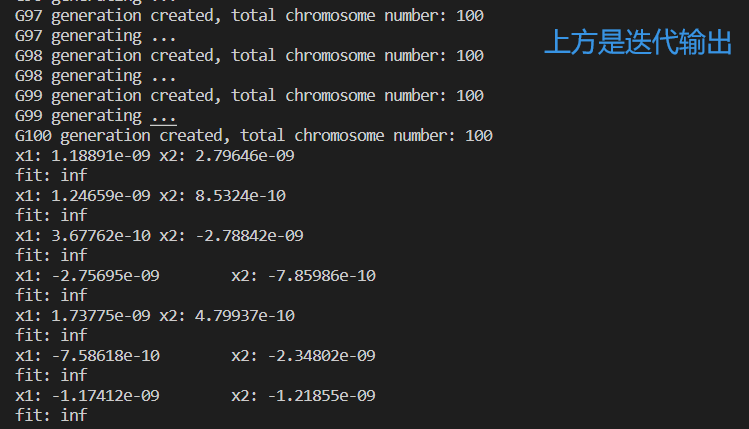
\includegraphics[width = 0.8\textwidth]{output_01.png}

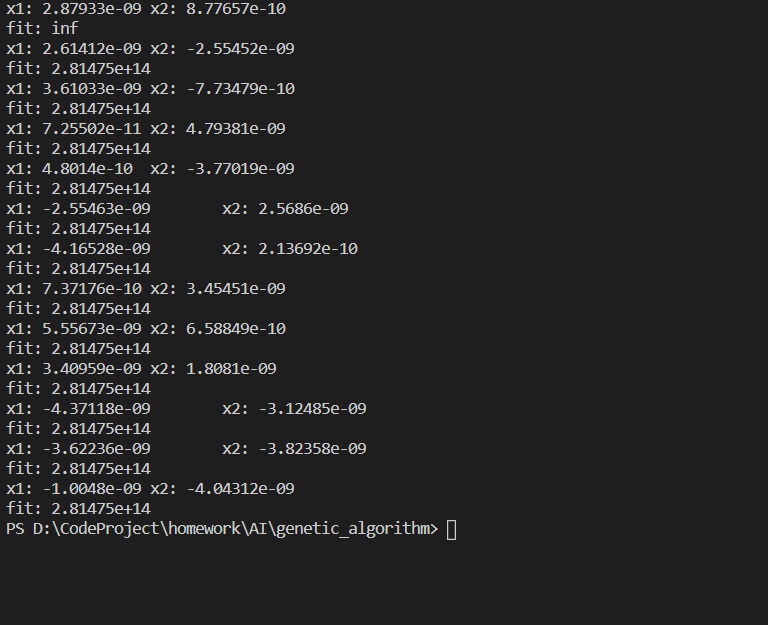
\includegraphics[width = 0.8\textwidth]{output_02.png}

可以看到,适应度最高接近无穷,
随着适应度的从低到高(输出是适应度从高到低),
x1和x2的值都有向0收敛的趋势。

但,仅仅从终端界面的输出也许并不方便看出数据的分布情况,
我们不妨使用matlab分阶段绘图。
给源代码增添一些文件输出的方法之后,修改main函数代码如下:

\begin{lstlisting}
int main {
    Chromosomeset chromosome_set;
    chromosome_set.create(20);
    chromosome_set.write( "g0.txt");

    chromosome_set.generate(2);
    chromosome_set.write("g2.txt");

    chromosome_set.generate(8);
    chromosome_set.write("g10.txt");

    chromosome_set.generate(40);
    chromosome_set.write("g50.txt");

    chromosome_set.generate(100);
    chromosome_set.write("g100.txt");
return 0;
}
\end{lstlisting}

将先后五次输出使用matlab绘制成为散点图,如下:

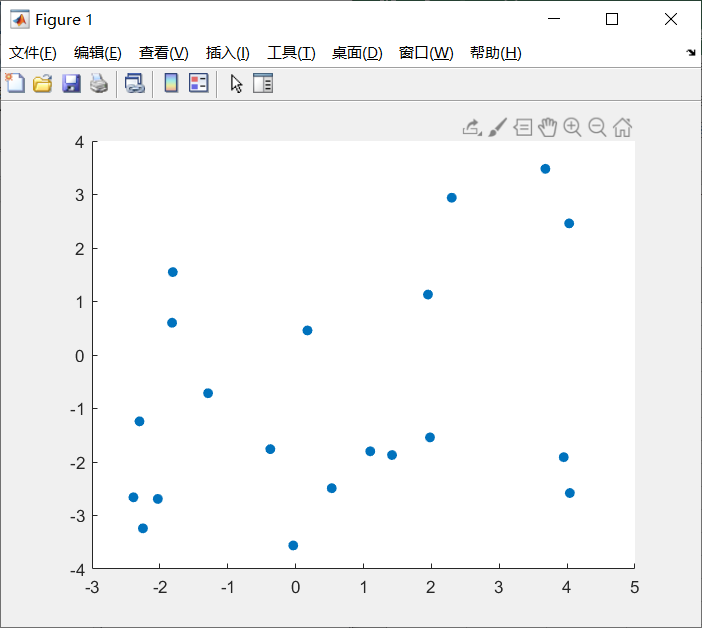
\includegraphics[width = 0.45\textwidth]{test1_01.png}
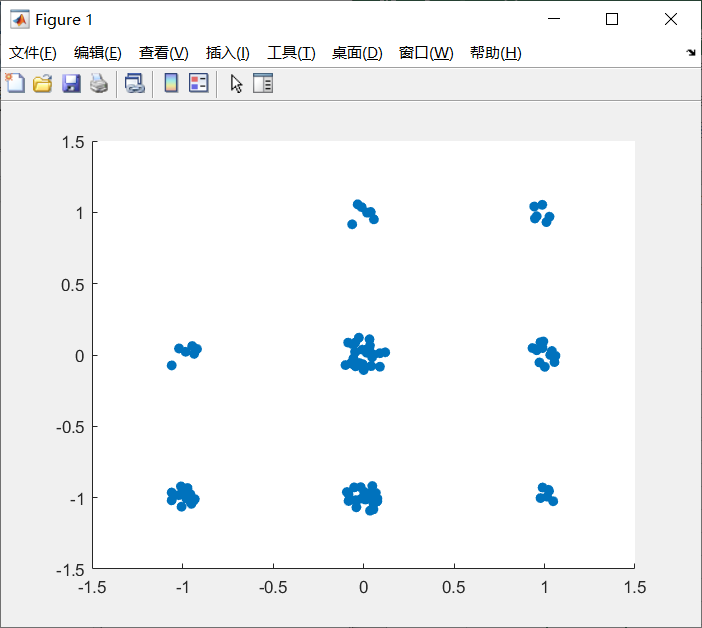
\includegraphics[width = 0.45\textwidth]{test1_02.png}

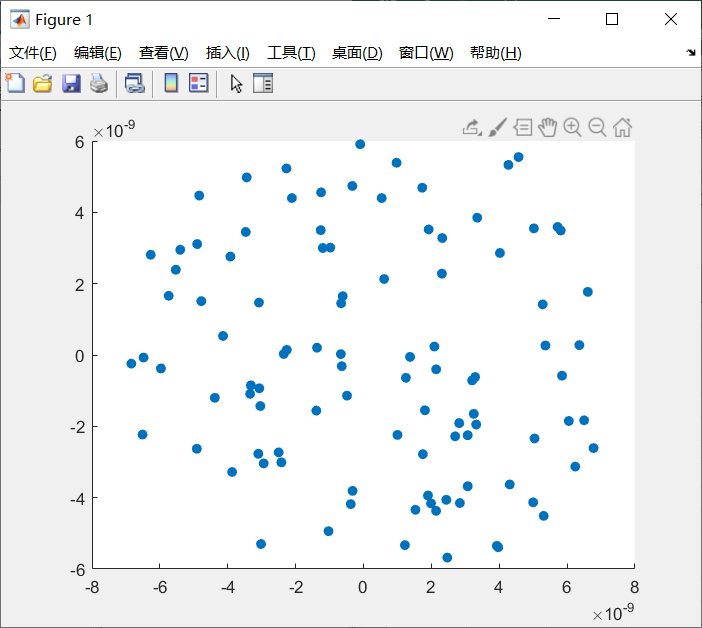
\includegraphics[width = 0.45\textwidth]{test1_03.png}
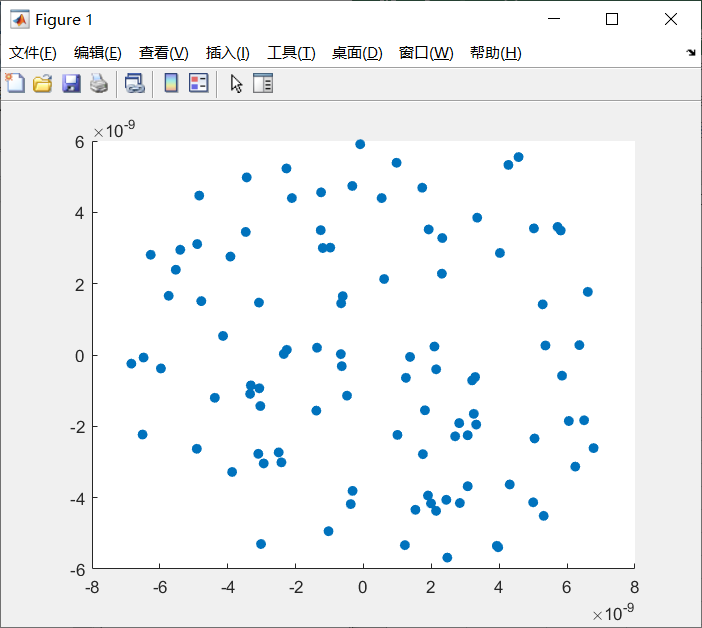
\includegraphics[width = 0.45\textwidth]{test1_04.png}

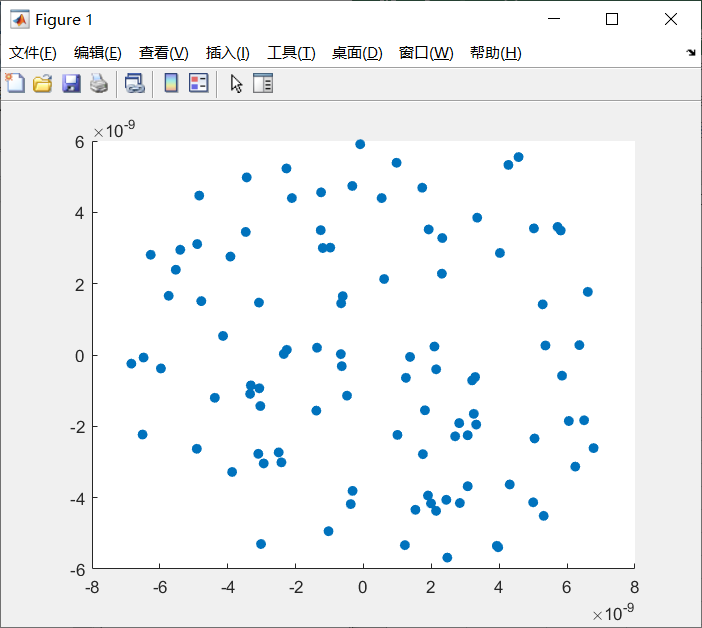
\includegraphics[width = 0.45\textwidth]{test1_05.png}

图片分别是迭代0次、2次、10次、50次、100次的输出。
可以发现,前三张散点图反映了粗略的迭代过程,
而迭代10次、50次、100次后输出的数据已经不再变化,
因为解的精度已经超出C++数据类型double可以处理的范围。

为了更好地观察迭代的过程,再进行一次实验,
这一次降低迭代的次数,增加输出的频率:

\begin{lstlisting}
int main () {
    ChromosomeSet chromosome_set;
    chromosome_set.create(20);
    chromosome_set.write("g0.txt");

    chromosome_set.generate(1);
    chromosome_set.write("g1.txt");
    chromosome_set.generate(1);
    chromosome_set.write("g2.txt");
    chromosome_set.generate(1);
    chromosome_set.write("g3.txt");
    chromosome_set.generate(1);
    chromosome_set.write("g4.txt");
    chromosome_set.generate(1);
    chromosome_set.write("g5.txt");

    chromosome_set.generate(5);
    chromosome_set.write("g10.txt");

    return 0;
}
\end{lstlisting}

将迭代0次、1次、2次、3次、4次、5次、10次的输出
按顺序分别绘制输出如下:

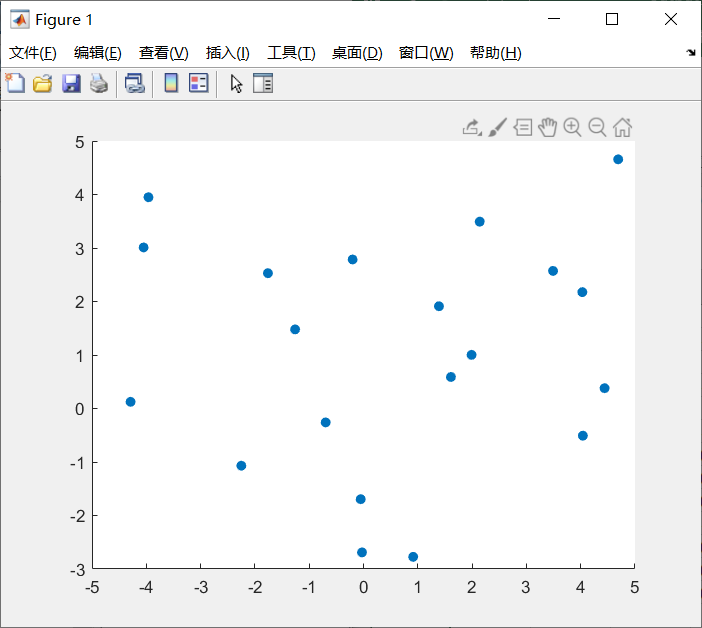
\includegraphics[width = 0.45\textwidth]{test2_01.png}
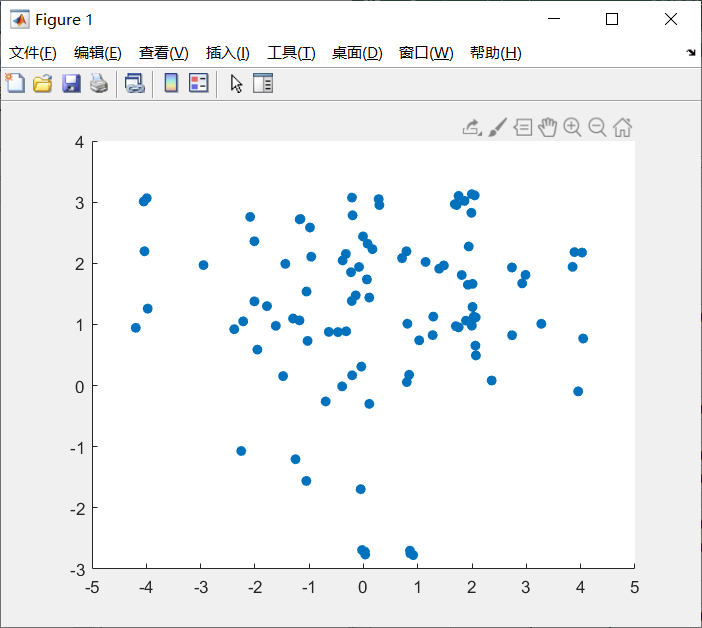
\includegraphics[width = 0.45\textwidth]{test2_02.png}

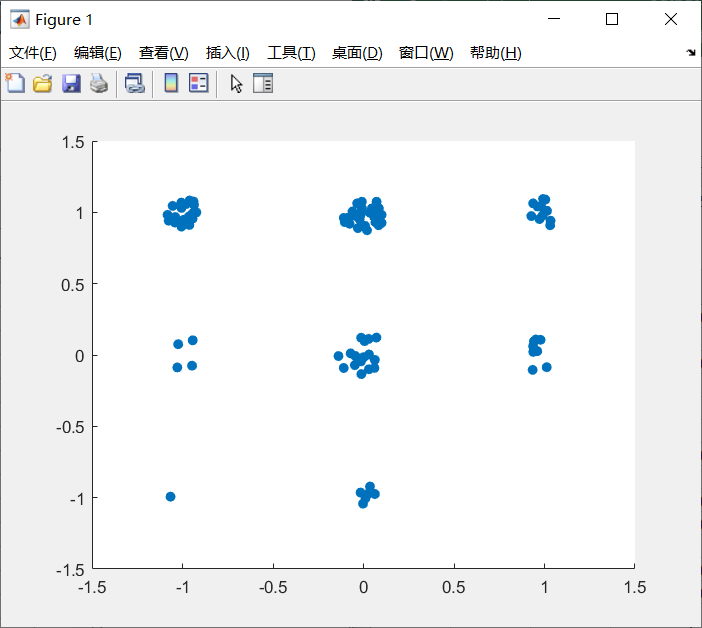
\includegraphics[width = 0.45\textwidth]{test2_03.png}
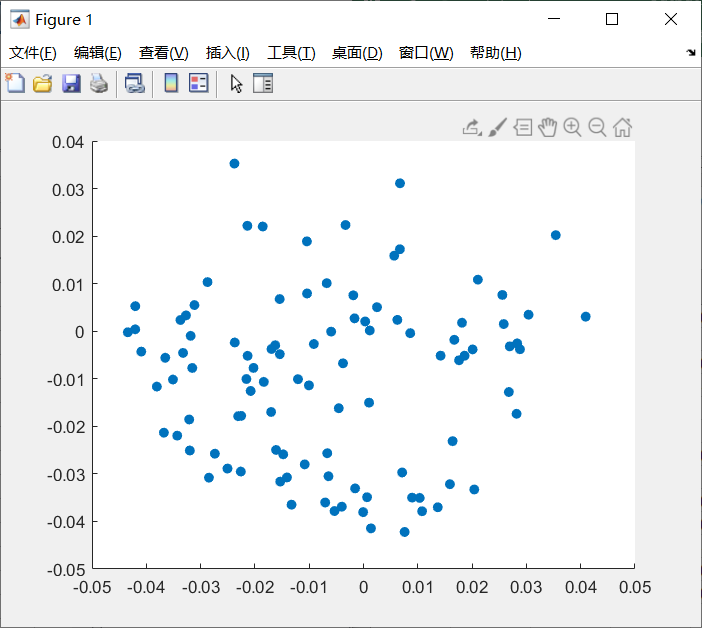
\includegraphics[width = 0.45\textwidth]{test2_04.png}

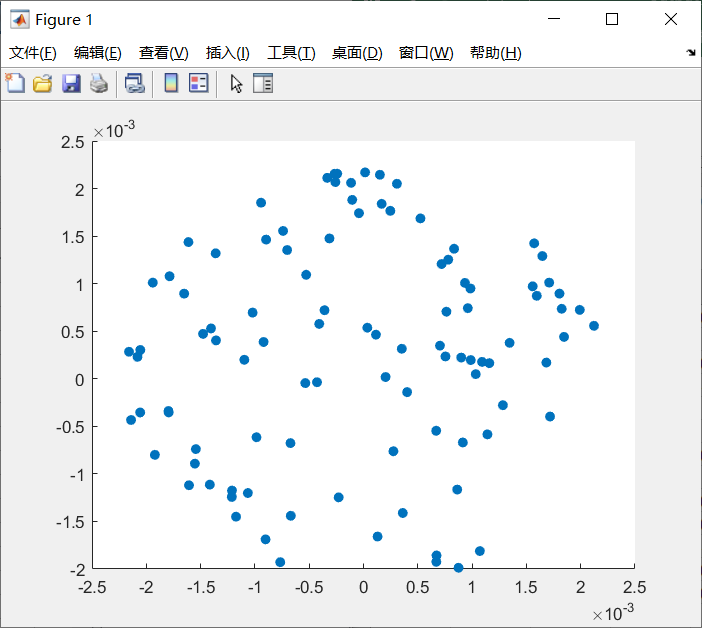
\includegraphics[width = 0.45\textwidth]{test2_05.png}
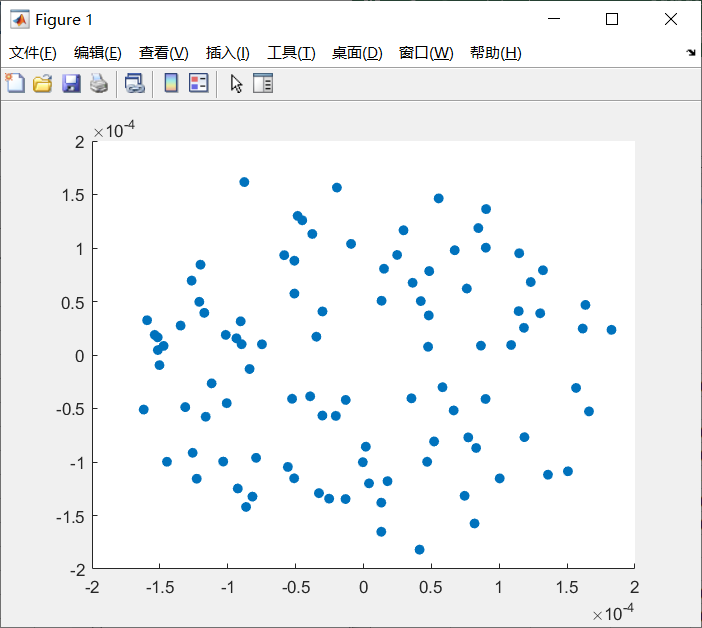
\includegraphics[width = 0.45\textwidth]{test2_06.png}

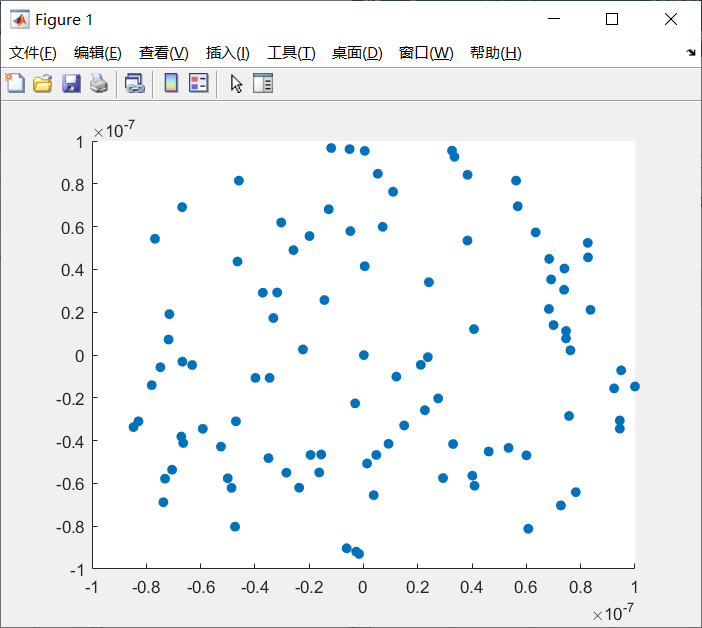
\includegraphics[width = 0.45\textwidth]{test2_07.png}

第三次迭代输出后解聚集在几个局部最优解附近,而第四次迭代之后,
所有局部最优解都被淘汰,并且从坐标轴刻度易知,
种群不断向(0,0)点进化。

通过上面的迭代并观察结果,可以明显发现每迭代一次,
解就在更靠近(0,0)点处聚集,
可以推测(0,0)点大概率(在某个精度的误差允许下)是函数的最小值点。
解有明显的向(0,0)点收敛的趋势。

\section{总结}

在实现算法时,应该先
通过理论分析构造算法过程,再转化为代码,
重点应该理解算法对遗传模拟的过程是如何在求解问题的过程中生效的。

使用面向对象的方法构建基因和基因集,将使代码构建的过程更加易于理解。
本次算法中的变异操作直接使用了随机,也许并不是很好的解决方案,
但最后的结果并没有受到影响。

通过对不同解的交叉、变异,生成一系列基因,
并保留最接近函数最优解(最小值)的基因,也许可以认为这类似一个反向的拟合过程。

遗传算法最终的输出也许并不会是最优解,而是一系列接近最优解的基因的集合。


\section{附录}

基因集的迭代函数具体实现如下:

\begin{lstlisting}
void ChromosomeSet::generate(int num) {
    int generation = 0;

    do {
        cout << "G" << generation << " generating ..." << endl;

        double total_fit = 0;
        for (Chromosome & c : this->_set) {
            double x1 = c.getX1();
            double x2 = c.getX2();
            double result = Function(x1, x2);

            c.setFit(1 / result);
            total_fit += 1 / result;
        }

        // Sort by fit descendingly.
        sort(_set.begin(), _set.end(),
            [](const Chromosome & c1, const Chromosome & c2) {
                return c1.getFit() > c2.getFit();
            });


        default_random_engine engine(time(nullptr));
        uniform_real_distribution<double> distribution(0, 1);

        vector<Chromosome> parent;
        for (long long unsigned int i = 0; i < _set.size(); ++ i ) {
            double rand_num = distribution(engine);
            double add_up = 0;
            for (Chromosome c : _set) {
                if (rand_num <= add_up) {
                    parent.push_back(c);
                }
                else {
                    add_up += c.getFit() / total_fit;
                }
            }
        }

        if (parent.size() % 2 != 0 ) parent.pop_back();

        for (auto iter = parent.begin(); iter < parent.end(); iter += 2) {
            for (auto c : Chromosome::crossover(* iter, *(iter + 1))) {
                double rand_num = distribution(engine);
                if (rand_num <= 0.001) c.mutate();

                double x1 = c.getX1();
                double x2 = c.getX2();
                double result = Function(x1, x2);

                c.setFit(1 / result);

                _set.push_back(c);
            }
        }

        // Sort by fit descendingly.
        sort(_set.begin(), _set.end(),
            [](const Chromosome & c1, const Chromosome & c2) {
                return c1.getFit() > c2.getFit();
            });

        while (_set.size() > _scale) {
            _set.pop_back();
        }


        ++ generation;
        cout << "G" << generation << " generation created, "
            << "total chromosome number: " << _set.size() << endl;
    } while (generation < num);
}
\end{lstlisting}

\begin{thebibliography}{99}
    \bibitem{ref 1}李德毅,于剑,中国人工智能协会.人工智能导论[M].中国科学技术出版社:北京,2018:72.
\end{thebibliography}

\end{document}